% TITLE: Lipsum text with two figures and math
% AUTHOR: Adrian Schrader
% Created on: 31/7/15

\section{Figures}
\subsection{Column wide figure}
\lipsum[1]
\lipsum*[2]\footnote{This is an unnecessary footnote. Thanks!}

\begin{figure}[h]
  \centering
  \includegraphics[width=\linewidth]{img/plot}
  \caption{Plot of of $ f(t) $ in Maple}~\label{img:function}
\end{figure}

\lipsum[3]
\lipsum[4]

\subsection{Page wide figure}
\lipsum[5]

\begin{figure*}[ht]
  \centering
  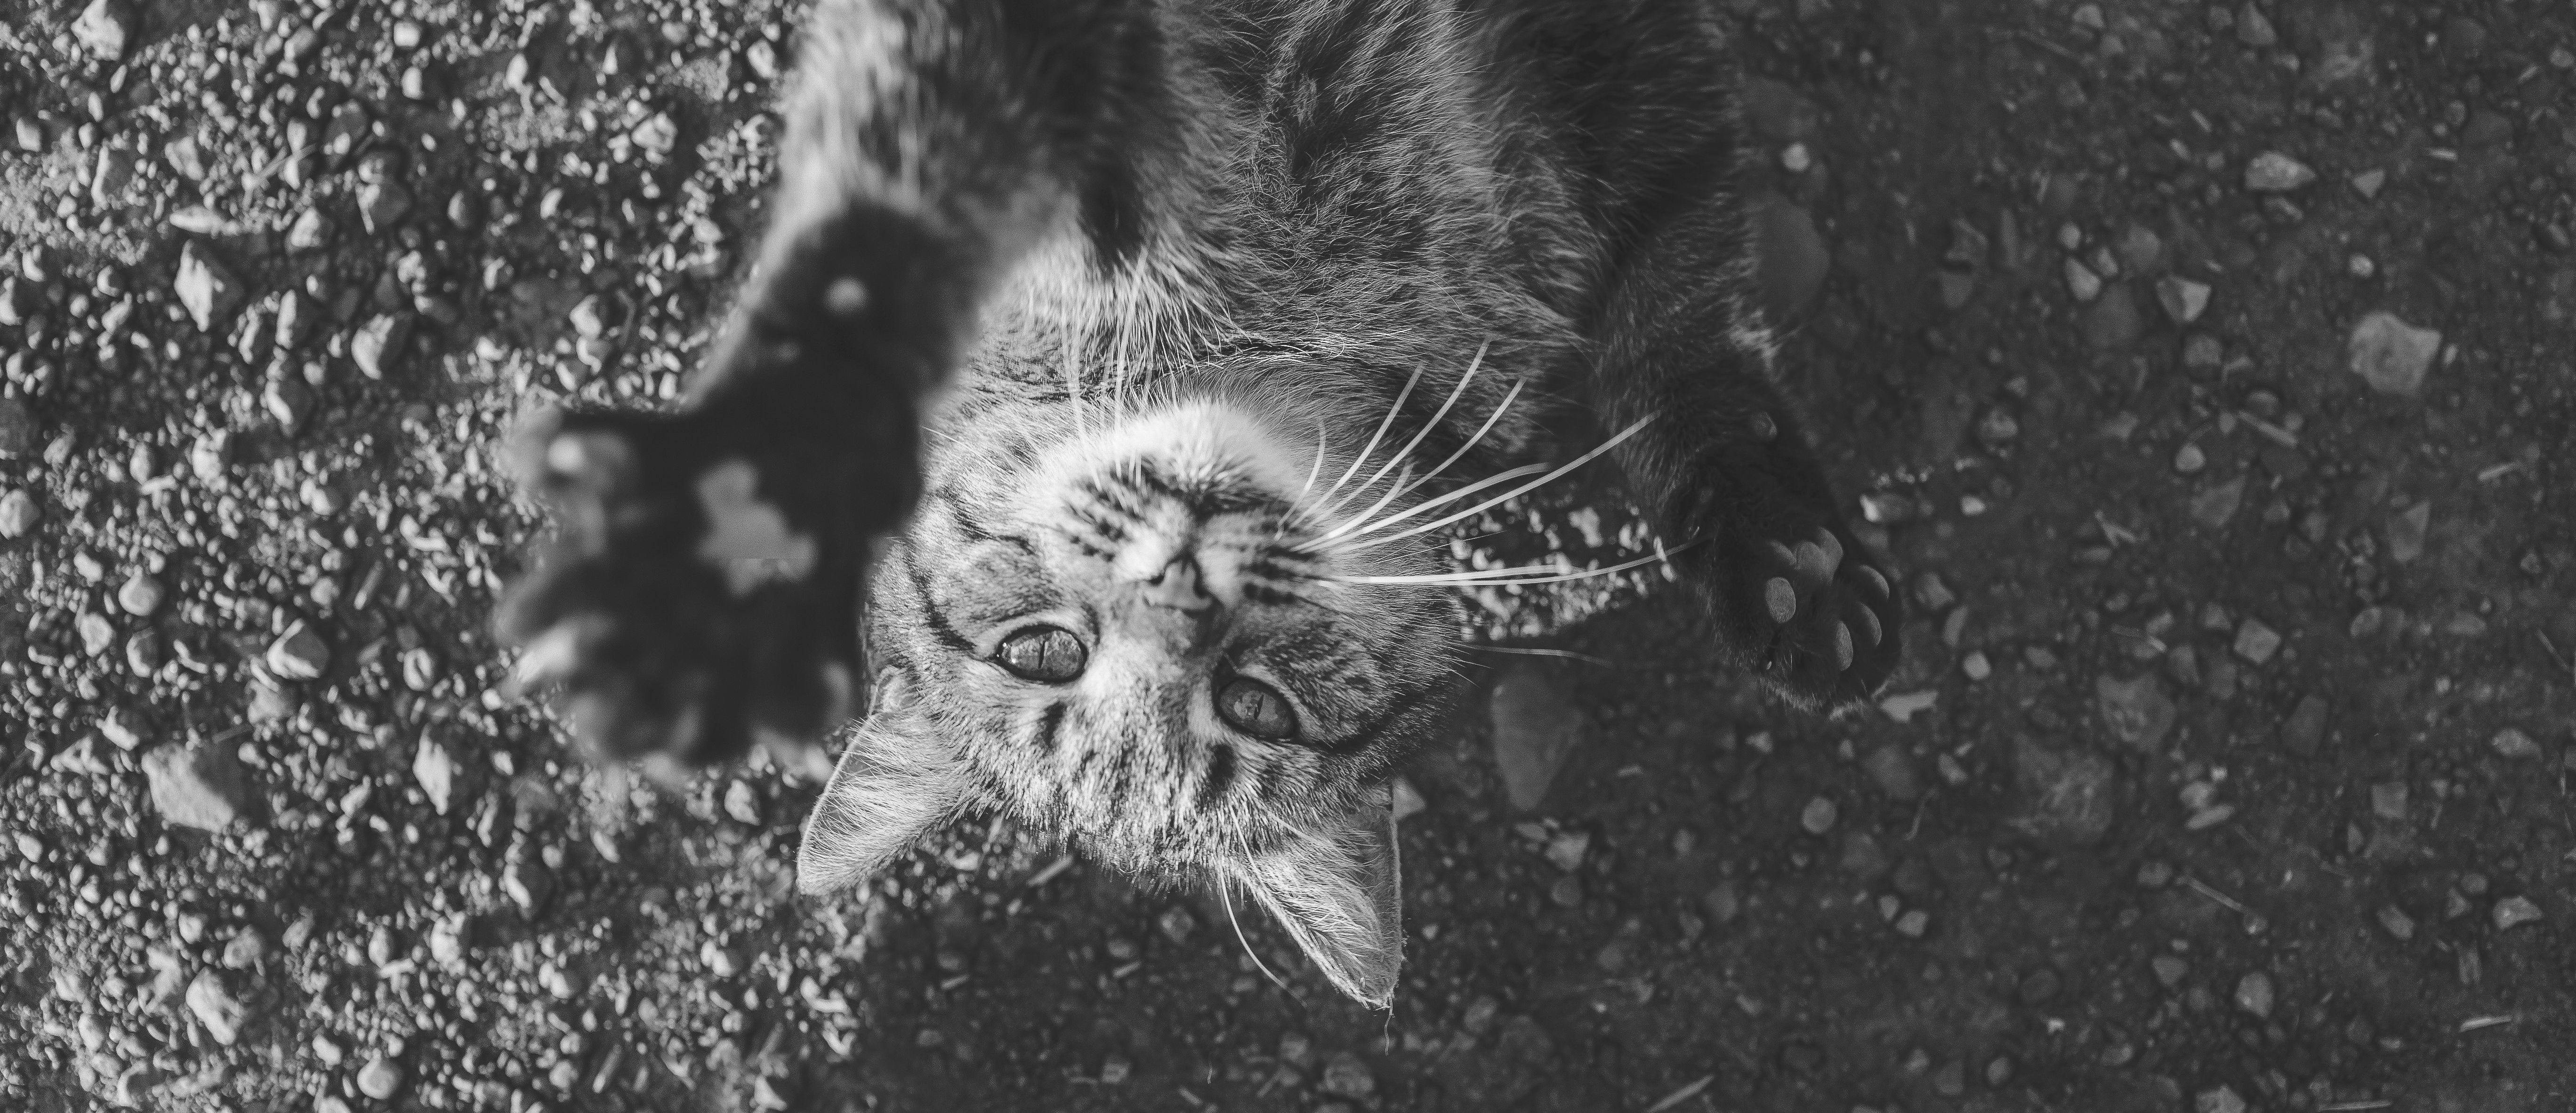
\includegraphics[width=\linewidth]{img/example2}
  \caption{Another Random cat picture from Google \protect\url{https://static.pexels.com/photos/4067/animal-pet-cute-cat.jpg}}~\label{img:cat2}
\end{figure*}

\section{Typesetting}
\lipsum[6]

\subsection{Formula and Equations}
\begin{align}
    f(t) &= s_0 \cdot e^{-\frac{t}{\tau}} \cdot \cos(\omega_s t) \cdot \Theta(t) \nonumber \\
    &= s_0 \cdot e^{-\frac{t}{\tau}} \cdot \frac{1}{2} \Big( e^{i \omega_s t} + e^{-i \omega_s t} \Big) \cdot \Theta(t)\\
    \tilde{f}(\omega) &= \mathcal{F}(f)(\omega) = \frac{1}{\sqrt{2\pi}} \int_{-\infty}^{\infty} f(t) \cdot e^{-i \omega t} dt \nonumber \\
    &= \frac{s_0}{\sqrt{2\pi}} \frac{\frac{1}{\tau} + i \omega}{ {( \frac{1}{\tau} + i \omega )}^2 + \omega_s^2}
\end{align}

\subsection{Source code}
\begin{listing}
  \begin{minted}{java}
    public static void main(String[] args) {
      return;
    }
  \end{minted}
  \caption{Standard main method of every java program}~\label{lst:javamain}
\end{listing}

\lipsum[9-14]
\lipsum[2]~\cite{book:handbook}
